\newpage

\section{Dataset}

The dataset used for this project was a competition dataset from Hugging Face, held in 2023 \cite{huggingface_competitions_aiornot}.
The dataset consists of 62,060 images, and is 2.37GB in size, being pre-split into training and tesing sets, as summarised in \cref{tab:dataset_summary,tab:class_counts}, where it can be seen that the testing set has the class labels withheld due to the competition setting, restricting this analysis to the 18,618 training images, which we can sub-divide and validate with known labels.
\begin{table*}[h]
    \centering
    \begin{minipage}{0.48\textwidth}
        \centering
        \begin{tabular}{ll}
            \toprule
            \textbf{Feature} & \textbf{Description} \\
            \midrule
            \code{id}     & Index filename \code{34.jpg} \\
            \code{image}  & The Image (512x512) \\
            \code{label}  & Binary class label \\
            \bottomrule
        \end{tabular}
        \caption{Dataset features and their descriptions.}
        \label{tab:dataset_summary}
    \end{minipage}\hfill
    \begin{minipage}{0.48\textwidth}
        \centering
        \begin{tabular}{lcc}
            \toprule
            \begin{tabular}[c]{@{}l@{}}\textbf{Class} \\ \textbf{Label}\end{tabular} & 
            \begin{tabular}[c]{@{}c@{}}\textbf{Train} \\ \textbf{Count}\end{tabular} & 
            \begin{tabular}[c]{@{}c@{}}\textbf{Test} \\ \textbf{Count}\end{tabular} \\
            \midrule
            AI (1)      & 10,330 $(55.5\%)$ & NA \\
            Not AI (0)  & 8,288 $(45.5\%)$ & NA \\
            \bottomrule
            \textbf{Total}       & 18,618 & 43,442 \\
        \end{tabular}
        \caption{Counts of each class label in the training and testing sets}
        \label{tab:class_counts}
    \end{minipage}
\end{table*}

The first step in the project involved preparing the dataset for training and evaluation. The dataset was initially loaded from HuggingFace and converted to NumPy arrays to enable further processing. A holdout set of 500 images was separated for final testing, with the size constrained by bandwidth limitations on the AWS endpoint, as discussed in \cref{sec:model_deployment}. 

The remaining data was split into three subsets: a small training set (10\%), a main training set (70\%), and a validation set (20\%), using HuggingFace's \code{train_test_split} method. To ensure class balance and avoid bias toward the majority class, \code{Imblearn}'s \code{RandomUnderSampler} was applied. This was required, because, as shown in \cref{tab:class_counts}, a model predicting only the majority class (AI-generated) could reach 55.5\% accuracy. 

The processed data was then saved as \code{.npz} files for efficient storage and loading, and uploaded to an S3 bucket to enable access during model training without being constrained by the RAM limits of the SageMaker notebook environment. \Cref{fig:s3_bucket} depicts a screenshot of the uploaded directories, each containing their respective \code{.npz} file. The data preprocessing code described above is provided in \cref{code:data_wrangling} in the appendix. 

\begin{figure}[h]
    \centering
    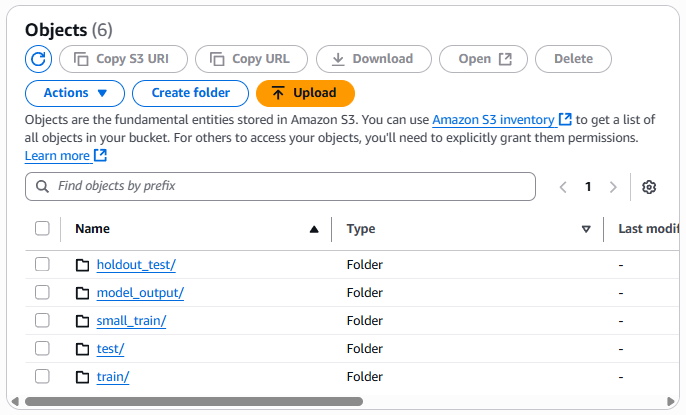
\includegraphics[width=250px]{figures/s3_bucket_screenshot.png} % Image filename
    \centering
    \caption{Screenshot of S3 Bucket with training data in AWS Console} % Caption
    \label{fig:s3_bucket} % Label
\end{figure}


